

\chapter{Inferential Roles Made Explicit}
%======================================================================
\renewcommand{\epigraphrule}{0pt}
\setlength{\epigraphwidth}{4.5in}
\epigraph{\textit{Logical vocabulary endows practitioners with the expressive power to make explicit as the contents of claims just those implicit features of linguistic practice that confer semantic contents on their utterances in the first place.}}{- Robert Brandom, 1994}

\section{Introduction}

It is a significant challenge to build a model that engages in intentionally interpretable behavior involving the use of natural language. One way to approach this challenge is to start with a model that a supports only a specific class of intentional state attributions, such as attributions of \textit{understanding} that concern specific linguistic expressions. Such attributions are in turn supported by the ability to infer what a given sentence follows from and is followed by \citep{Brandom:1994}. For example, to understand the sentence ``The dancers parade down the street,'' a model must be able to infer that the dancers are outside, that they are not standing still, that there is likely a surrounding audience, along with a variety of other things. And since understanding a sentence involves understanding its \textit{meaning}, it follows from this view that the meaning of an expression is determined by the inferences it licenses \citep{Brandom:1994,Sellars:1953,Sellars:1954,Brandom:2000,Brandom:2009}. 

An important feature of this view is that it tightly couples the meaning of a linguistic expression to the role the expression plays in practices that involve intentional interpretation. It is accordingly possible to derive an explicit characterization of an expression's meaning from the structure of a model that can be successfully interpreted using intentional vocabulary. To explain, if a model can be correctly attributed an intentional state of the form ``\textit{X} understands \textit{Y}'', then the inferential behavior of the model that licenses this attribution essentially charts out the inferential role that constitutes the meaning of the expression \textit{Y}. As such, one way to achieve the goal of a technically rigorous inferential role semantics is to build an intentionally interpretable model that draws the same inferences that a competent language user would.

To work towards this goal, I introduce a neural network model that learns to generate sentences that are the inferential consequences of its inputs. The model functions by first encoding a sentence into a distributed representation, and then decoding this representation to produce a new sentence. The encoding procedure involves dynamically generating a tree-structured neural network of the sort depicted in Figure \ref{depnet}. Once a sentence encoding is produced using this network, it is fed through an ``inverse'' tree-structured network to produce a predicted sentence. Interestingly, different inverse or decoding networks can be used to generate different sentences from a single encoding. To train the model parameters (i.e., the network weights shared across different tree structures) I use the Stanford Natural Language Inference (SNLI) dataset \citep{Bowman:2015}. Overall, the purpose of the model is to formally specify or ``make explicit'' the inferential roles of arbitrary linguistic expressions \citep{Brandom:1994}. The model achieves this purpose by assigning a rough likelihood to every sentence that is a potential inferential consequence of its input. 

In what follows, I first describe the model and then empirically evaluate its ability to produce plausible entailments for sentences unseen in its training data. I present experimentally produced plausibility ratings for a random collection of generated sentences, and from these ratings conclude that the model captures something important about the inferential roles of ordinary linguistic expressions. Next, I provide a number of more qualitative evaluations of the model that involve (a) iterating its predictions to produce chains of inferences \citep{Kolesnyk:2016}, (b) performing word-level input substitutions to determine the inferential significance of subsentential expressions \citep{Brandom:2000,Brandom:1994}, and (c) conditioning the model's predictions on additional inputs in the form of simple prompts and questions. I then provide a discussion of possible extensions of the model that would enable it to function as a more sophisticated intentional system \citep{Dennett:1991,Dennett:1987}. I conclude that if such extensions were realized, the model's behavior would be largely indistinguishable from that of a competent speaker who knows the meanings of all the expressions that make up a particular language.

\section{Model Architecture}

The model itself is a variant of the tree-structured neural network described in Chapter 2. For this reason, I briefly review the details of these networks before introducing the specific architecture I use to generate the inferential consequences of arbitrary input sentences. The basic idea behind this architecture, familiar from machine learning research on sequence transduction \citep{Sutskever:2014}, is to use one neural network to ``encode'' a sentence into an embedding, and use a second neural network to ``decode'' a new sentence from this embedding. Here, the aim is to make the decoded sentence be an inferential consequence of the encoded sentence. Related ideas can be found in the work of Iyyer et al. (\citeyear{Iyyer:2014}) and Kolesnyk et al. (\citeyear{Kolesnyk:2016}).

\subsection{Tree-Structured Models Revisited}

To start, recall that a tree-structured neural network is designed to merge distributed representations of words into distributed representations of phrases and sentences \citep{Socher:2012,Socher:2014}. Three steps are involved in this process. First, a parser is used to derive a parse tree from some sentence of interest. Second, this tree is transformed into a neural network by replacing its edges with weights and its nodes with layers of artificial neurons. Third, activation is propagated up the tree by providing input to layers that correspond to certain nodes, as shown in Figure \ref{depnet}. The input at each node is typically a distributed representation or ``embedding'' corresponding to a single word \citep{Mikolov:2013,TurneyPantel:2010,Sahlgren:2008}.

\begin{figure}[t]
\begin{center}
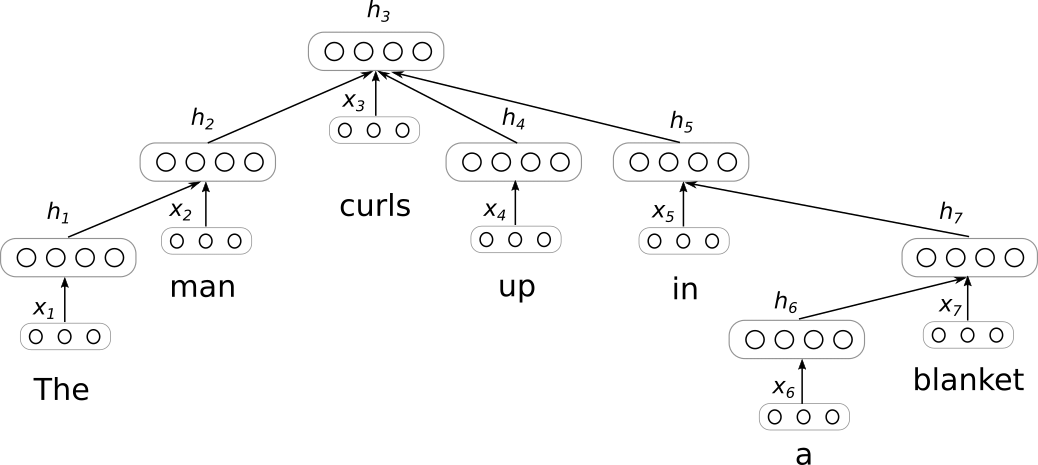
\includegraphics[width=4in]{figures/depnet.png}
\end{center}
\caption{Sentence encoding with a dependency-based tree-structured neural network. A dependency parser is used to produce the computational graph for a neural network, which is then used to produce an embedding of a sentence by merging embeddings of individual words. Figure adapted from Socher et al. (\citeyear{Socher:2014}).} 
\label{depnet}
\end{figure}

It is possible to apply these methods using arbitrary tree structures, and I adopt a dependency-based syntax in the experiments described below. There are three reasons for this choice \citep{Socher:2014}. First, the assignment of different network weights to different dependency relations allows for the creation of networks that are more sensitive to syntactic information. Second, the semantic role of an individual word can often be read off of the dependency relation it bears to a head word, which allows for the creation of networks that are also sensitive to semantic information. Finally, dependency trees are less sensitive to arbitrary differences in word order, which helps to ensure that simple variations of a sentence get mapped to similar distributed representations. The specific model I adapt -- the dependency-based tree-structured neural network -- is introduced in Socher et al. (\citeyear{Socher:2014})

It is worth briefly summarizing the process by which this model is used to generate sentence embeddings. First, an input sentence $s$ is converted into a list of pairs, such that $s = [(w_1, x_1)...(w_n, x_n)]$, where $w$ is a word and $x$ is the corresponding word embedding. Next, a dependency parser is used to produce a tree that orders the words in the sentence in terms of parent-child relations. Each node in this tree is then assigned an embedding, $h_i$, in a two-step manner that is described more formally in the previous chapter. First, all of the leaf nodes in the tree (i.e., nodes that do not depend on other nodes) are assigned embeddings by applying a simple transformation to their underlying word embeddings. Second, embeddings are recursively assigned to all of the non-leaf nodes by composing the embeddings of their children. So, in the example tree in Figure \ref{depnet}, the embeddings for nodes 1, 4, and 6 would be computed first, since these nodes have no children. Then, embeddings will be computed for any nodes whose children now all have assigned embeddings (in this case, nodes 2 and 7). And so on, until an embedding is computed for every node.

Model training is done via backpropogation and requires that a cost function be defined for the sentence embeddings produced at the root of each tree. The free parameters are the weights and biases associated with each dependency, along with a single embedding matrix $W_v$. Word embeddings can also be fine-tuned over the course of training. The number of dependency relations, and hence the number of weight matrices in the model, depends on the specific syntactic formalism that is used. In the experiments described below, 45 dependency relations define the syntax that is used by the model's parser.

\subsection{Cost Functions For Entailment Generation}

Choosing an appropriate cost function for a tree-structured neural network can be difficult, since it is not always clear what makes for a ``good'' sentence embedding. It is accordingly common to see tree-structured networks applied to narrow classification tasks such as the prediction of sentiment ratings \citep[e.g.,][]{Socher:2012}. My goal is to define an optimization objective that accounts for the principle that understanding a linguistic expression involves drawing certain inferences.

To accomplish this goal, I define a model composed of two tree-structured networks, one that encodes an input sentence into a distributed representation, and another that decodes this representation into a new sentence that is entailed by the input sentence. This model is inspired by Iyyer et al.'s (\citeyear{Iyyer:2014}) work using tree-structured networks analogously to autoencoders, but introduces a decoding procedure that computes an appropriate response to the input sentence, rather than merely reconstructing it. Figure \ref{decoder} provides an illustration of this pairing of encoder and decoder networks.

The model is trained on pairs of sentences standing in entailment relations. A dependency parser\footnote{I use the SpaCy python library, available at https://spacy.io} is used to produce a tree-structured network for each sentence, but the network associated with the second sentence is run in reverse, as shown in Figure \ref{decoder}. A word prediction is generated at each node in this second tree using a softmax classifier, which makes it possible to define a cross-entropy loss over nodes and trees as follows: 

\begin{align}
J(\theta) = - \sum_{i} \sum_{j} t^{(i)}_j \log{ p(c^{(i)}_j | s_i)}
\end{align}

\noindent
where $t^{(i)}_j$ is the target probability (i.e. 1) for the correct word at the $j^{th}$ node in the $i^{th}$ training example, $p(c^{(i)}_j | s_i)$ is the computed probability for this word given the input sentence $s_i$, and $\theta$ is the set of combined parameters for the encoder and decoder networks. Intuitively, this cost function penalizes model parameters that fail to assign a high joint probability to the collection of word predictions in the decoder that correspond to the correct entailment for a given input sentence. More formally, the training objective is to maximize the log probability of the example entailments provided in the training data. 

\begin{figure*}[t]
\begin{center}
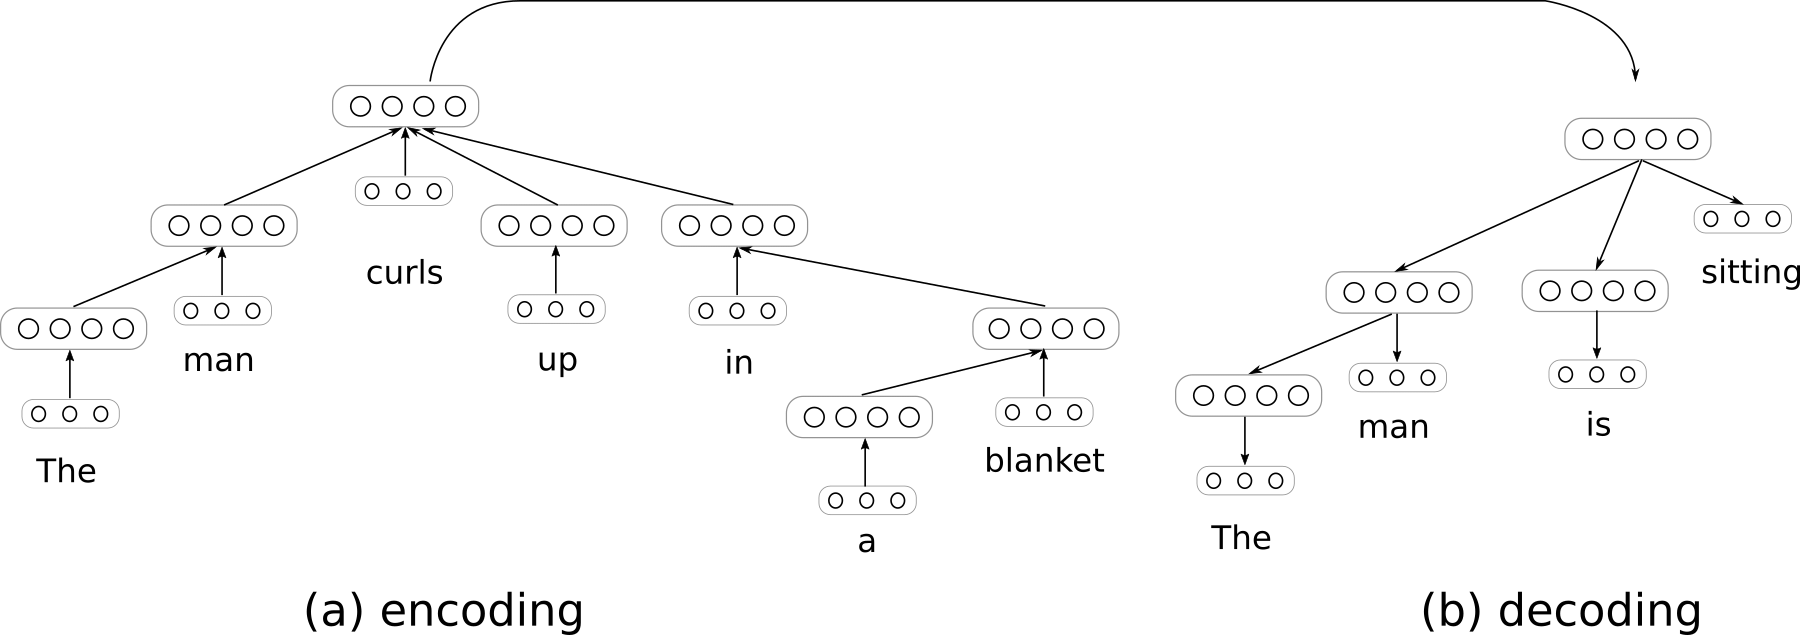
\includegraphics[width=5.5in]{figures/decoder.png}
\end{center}
\caption{Generating entailments with paired encoder and decoder neural networks. The decoder network computes a probability distribution over words at each node, conditioned on the sentence representation produced by the encoder. The parameters of both the encoder and decoder are trained via backpropogation through structure using error derivatives supplied at each node in the decoding tree. The encoder and decoder trees are dynamically generated for each pair of sentences in the training data. During inference, it is possible to use different decoding trees to generate different entailments from a single sentence encoding.} 
\label{decoder}
\end{figure*}

I train the model via stochastic gradient descent by backpropogating through both the decoder and encoder tree for each training example. The result of training is a set of weights associated with dependencies for both encoding and decoding, a set of weights for predicting a distribution over words from a node embedding for each dependency, the bias $b$ in each network, and the input transformation matrix $W_v$. When the trained model is used to perform inference using a novel input sentence, the encoder network is assembled into a tree using the learned encoding weights. The decoder network is then also assembled into a tree using the learned decoding weights, and activation is propagated through the encoder and into the decoder to produce a probability distribution over words at each tree node. The words with the highest probability at each node are then used to construct the predicted entailment for the input sentence. The tree structure for the decoder can either be selected randomly or stipulated ahead of time. 

\section{Experiments}

To evaluate the model, I perform a number of experiments that illustrate how it assigns inferential roles to arbitrary linguistic expressions. The first experiment provides a quantitative assessment of how well the model is able to learn from examples of correct inferential transitions between sentences. Specifically, for a set of novel test sentences, I measure the percentage of correct word-level predictions relative to the ``ground truth'' entailments for these test sentences present in the dataset. The second experiment provides an empirical assessment of the plausibility of entailments generated by the model for a random selection of novel test sentences. Very roughly, human subjects are asked to rate the likelihood that model-generated entailments are true given that the sentences provided as inputs to the model are also assumed to be true. Together, these two experiments provide a fairly rigorous measure of how well the model is able to generate sentences that are the inferential consequences of its inputs.

The remaining assessments of the model are accordingly more qualitative in nature. The third experiment, following Kolesnyk et al. (\citeyear{Kolesnyk:2016}), involves iterating the encoding-decoding procedure to generate chains of entailments from a given input sentence. Interestingly, this sort of iteration can be used to explicitly build out inferential roles for arbitrary input sentences, as illustrated in Section \ref{sec:iteration} below. The fourth experiment involves substituting individual words in an input sentence to identify whether the model is able to ``interpolate'' between known examples of correct inferential transitions to produce novel transitions that are nonetheless correct. A further goal of this substitutional analysis is to evaluate the extent to which the model is able to learn word-level indirect inferential roles of the sort discussed by Brandom (\citeyear{Brandom:1994}). The final experiment is the most speculative in nature, and is designed to condition the model's generation of an entailment on a further input such as a prompt or a question. The goal of this experiment is to evaluate the extent to which the model is able to selectively navigate the inferential roles is assigns to particular sentences. If successful, this kind of selective navigation provides a foundation for more complicated forms of question-answering that many researchers take to be at the core of intelligence \citep{Weston:2015,Weston:2016}. 

\subsection{Model Training}

To train the encoder and decoder components of the model, I use a subset of the SNLI dataset \citep{Bowman:2015}. Each pair of sentences in this dataset is labeled with a particular inferential relationship, as discussed in the previous chapter. Since my interest is in generating entailments, I only consider pairs labeled with the entailment relation. To reduce the amount of noise and complexity in the dataset, I also perform some simple pre-processing. First, I screen for misspelled words,\footnote{I use the PyEnchant python library, available at http://pythonhosted.org/pyenchant/.} and eliminate all sentence pairs containing a misspelling. The resulting vocabulary for the model consists of 25,550 words. Second, I eliminate all sentence pairs containing a sentence longer than 15 words in order to avoid fitting model parameters to a small number of very long sentences that produce highly complex dependency trees. After preprocessing, the data consists of a 106,288-pair training set, a 1701-pair development set, and 1666-pair test set. The training set is used for learning model parameters, while the development set is used to tune hyperparameters such as the learning rate and the number of training epochs.

\begin{table}[!t]
\begin{center} 

\caption{Examples of Entailments Generated From Novel Test Sentences.} 

\label{examples}
\vskip 0.06in
\setlength{\tabcolsep}{12pt}
\begin{tabular}{ll} 
\hline

\multicolumn{1}{c}{\rule{0pt}{3ex} INPUT SENTENCE} & 
\multicolumn{1}{c}{GENERATED ENTAILMENT} \\

\hline
% \setlength{\tabcolsep}{1pt}
\rule{0pt}{3ex}The man in colorful shorts is barefoot. & The man is wearing his shorts. \\
A young man sleeping next to a dog. & A man is near a dog. \\
The 3 dogs are cruising down the street. & The dogs are on the street. \\
Woman reading a book with a grocery tote. & A woman with book is reading. \\
\hline
\end{tabular}
\end{center} 
\end{table}

Prior to training, the word vectors that are used as input to the encoder are initialized as 300-dimensional word2vec embeddings \citep{Mikolov:2013}. Each set of weights associated with a syntactic dependency is initialized as a $300 \times 300$ identity matrix with mean-zero Gaussian noise for both the encoder and decoder. The word transformation matrix, $W_v$, is initialized in the same way. During learning, all of these matrices are updated using stochastic gradient descent, along with the word2vec embeddings. Approximately 10 passes through training data are performed using an initial learning rate of $2 \times 10^{-4}$. The learning rate is progressively annealed over the course of training.

As an initial illustration of the kind of model performance this training results in, Table \ref{examples} provides some examples of entailments produced for sentences drawn from the SNLI test set. The decoding trees used to produce each of these entailments are chosen randomly, which indicates that the model is capable of learning to produce sentences with novel syntactic properties. It is also worth noting that each example here is only the \textit{most probable} entailment given a particular decoding tree. It is therefore theoretically possible to compute ranked collections of entailments with each decoding tree.  

\subsection{Evaluating Entailment Accuracy}

Recall that the SNLI corpus consists of pairs of sentences, and that the first sentence in each pair is referred to as the ``premise'' while the second sentence is referred to as the ``hypothesis''. In the procedure just described, the model is essentially learning to predict the hypothesis paired with each example premise in the training data. It is therefore possible to measure how accurately the model performs this task. Specifically, one can measure the proportion of nodes in the model's decoder for which the predicted word is the same as the correct word in the relevant hypothesis sentence. A caveat is that the tree for this sentence must be provided to the decoder, such that input activities are propagated through paired trees of the sort depicted in Figure \ref{decoder}, where the decoder tree is the correct tree for the conclusion of the inferential transition being considered.

When applied to the training set, this accuracy measure indicates the extent to which the model has ``memorized'' the example inferential transitions it was presented with during learning. When applied to the test set, the measure indicates whether the model has learned something that allows it to correctly predict specific inferential transitions in novel situations. It is worth noting that this measure is not entirely ideal in the case of the test set, since the model might generate a plausible entailment from a premise sentence that is non-identical to the specific entailment that is present in SNLI. It is also worth noting that prior work involving SNLI has almost uniformly focused on the problem of classifying sentence pairs. As such, I cannot easily draw comparisons to earlier work.

\begin{table}[!t]
\begin{center} 
\caption{Word-Level Accuracy for Entailment Generation} 
\label{accuracy} 
\vskip 0.12in
\begin{tabular}{c c c} 
\hline
Model  &  Training Set (\%)  & Test Set (\%)\\
\hline
\rule{0pt}{3ex}Chance  &  6.0 &  5.9 \\
Encoder-Decoder  &  66.7 & 61.8  \\
\hline
\end{tabular} 
\end{center} 
\end{table}

The results of computing entailment generation accuracies on the both training and test sets are presented in Table \ref{accuracy}. A baseline accuracy computed by chance is also reported. The model performs considerably better than chance, both because it has a large number of free parameters and because it is able to use syntactic information to condition its word predictions on part-of-speech information implicit in the structure of a decoding tree. For example, if the tree requires a particular word to be a determiner, then the number of plausible candidate words shrinks drastically, since there are only a handful of determiners in English (e.g., ``the'', ``a'', etc.). The model also generalizes surprisingly well to novel test sentences, with a fairly limited drop in accuracy.\footnote{If the model were merely memorizing the example inferential transitions present in the training data, then this drop would likely be much higher due to overfitting.} One point to note concerning this generalization is that extremely high accuracies on the test set are not entirely desirable, since they would indicate that the model has learned to exclusively predict a specific inferential transition for each input sentence. However, there are numerous examples of correct inferential transitions involving such sentences, and the model should ideally be learning to assign a high likelihood to all of them.  

Overall, the fact the model can generate the example inferential transitions in SNLI with a fairly high degree of accuracy provides good initial evidence that it is able to codify the inferential roles of ordinary linguistic expressions. Examples of the sort listed in Table \ref{examples}, moreover, suggest that these inferential roles are comprised of well-formed sentences that a competent speaker of English could readily understand. 

\subsection{Evaluating Entailment Plausibility}

One limitation of the assessments just described is that they do not provide a quantitative measure of how plausible or comprehensible the sentences produced by the model are. I therefore perform a simple study in which human subjects are asked to evaluate the plausibility of model-generated sentences. During the study, participants are shown a series of sentences introduced as true captions of unseen images.\footnote{Recall that all of the sentence pairs in SNLI were generated by providing subjects with a caption for an unseen image and asking them to produce a further caption that is either true, false, or maybe true of the image. So all of the sentences in SNLI can be described as image captions. The point of using this caption-based strategy in the construction of the dataset is to eliminate co-reference ambiguities that make it difficult to determine the appropriate inferential relationship between two sentences. See Bowman et al. (\citeyear{Bowman:2015}) for more details.} For each caption, the participants are shown an alternate caption and asked to evaluate the likelihood that it is also true of the corresponding image. Evaluations are recorded using a five point Likert scale that ranges from ``Extremely Unlikely'' (1) to ``Extremely Likely'' (5). The original caption in each case is the first sentence in a pair randomly chosen from the SNLI test set, while the alternate captions are either (a) model-generated entailments, (b) human generated entailments drawn from the test set, or (c) human generated contradictions also drawn from the test set. Participants are divided into three separate conditions corresponding to each type of alternate caption. This between-subjects experimental design is similar to the method used by Bowman et al. (\citeyear{Bowman:2015}) to validate human-generated sentence pairs during the creation of SNLI. The main difference is that model-generated sentences are evaluated in addition to human-generated sentences. 

\begin{table}[!t]
\begin{center} 
\begin{threeparttable}

\setlength{\tabcolsep}{16pt}

\caption{Plausibility Ratings for Inferential Relations.} 
\label{ratings} 
\vskip 0.12in
\begin{tabular}{c c c} 
\hline
Source & Status &  Mean Likert Rating (1-5) \\
\hline
\rule{0pt}{3ex}Human & Entailment  &  4.05  $\pm$ 0.09 \\
Model & Entailment  &  3.53 $\pm$  0.12 \\
Human & Contradiction & 2.05 $\pm$ 0.12 \\

\hline
\end{tabular}
\begin{tablenotes}
      \vskip 0.06in
      \footnotesize
      \item\centering * Margins are bootstrapped 95\% confidence intervals.
\end{tablenotes}

\end{threeparttable}
\end{center} 
\end{table}

Seventy-five participants from the United States were recruited through Amazon's Mechanical Turk and split evenly into the three conditions.  The main captions were identical across conditions, and each participant was asked to rate 20 caption pairs.\footnote{Two of the main captions had no associated contradictions in SNLI, so subjects in the contradiction condition only rated 18 captions.} Participants were paid \$1.00 for their time. Two participants failed to complete the study and did not have their responses included in the results. Repeat participation was blocked by screening Mechanical Turk worker IDs. 

The Likert ratings collected during the study are assessments of the plausibility of the inferential transition from one sentence (the main caption) to another (the alternate caption). The transitions involving sentence pairs drawn directly from SNLI offer a kind of gold standard for both good and bad transitions. The results shown in Table \ref{ratings} indicate that model-generated transitions are seen to be almost as plausible as the gold-standard transitions drawn from SNLI. As such, this study provides important evidence in support of the claim that the model is able to capture certain tacit inferential relationships between natural language expressions: the inferential relationships charted out by the model are seen to be nearly as truth-preserving as those charted out by competent language users. 

\subsection{Iteration Analysis}\label{sec:iteration}

Once an input sentence has been passed through the model to generate an entailment, it is possible to use this entailment as a new input to the model. Repeated applications of the model accordingly make it possible to chart out an ``inferential network'' around a particular starting sentence. Figure \ref{inf-gen} presents a simple example of an inferential network in which the sentence ``Some kids are wrestling on an inflatable raft'' is mapped onto a number of its inferential consequences. An important difference between this inferential network and the one shown in the previous chapter is that this network is generated directly from a single input sentence. Before, the network was constructed by testing large numbers of candidate sentences to see whether they are predicted to follow from a given input sentence. Figure \ref{chain} presents a slightly different example in which various sentences describing men doing things outdoors are eventually mapped onto the sentence ``A man is outdoors.''

\begin{figure*}[t]
\begin{center}
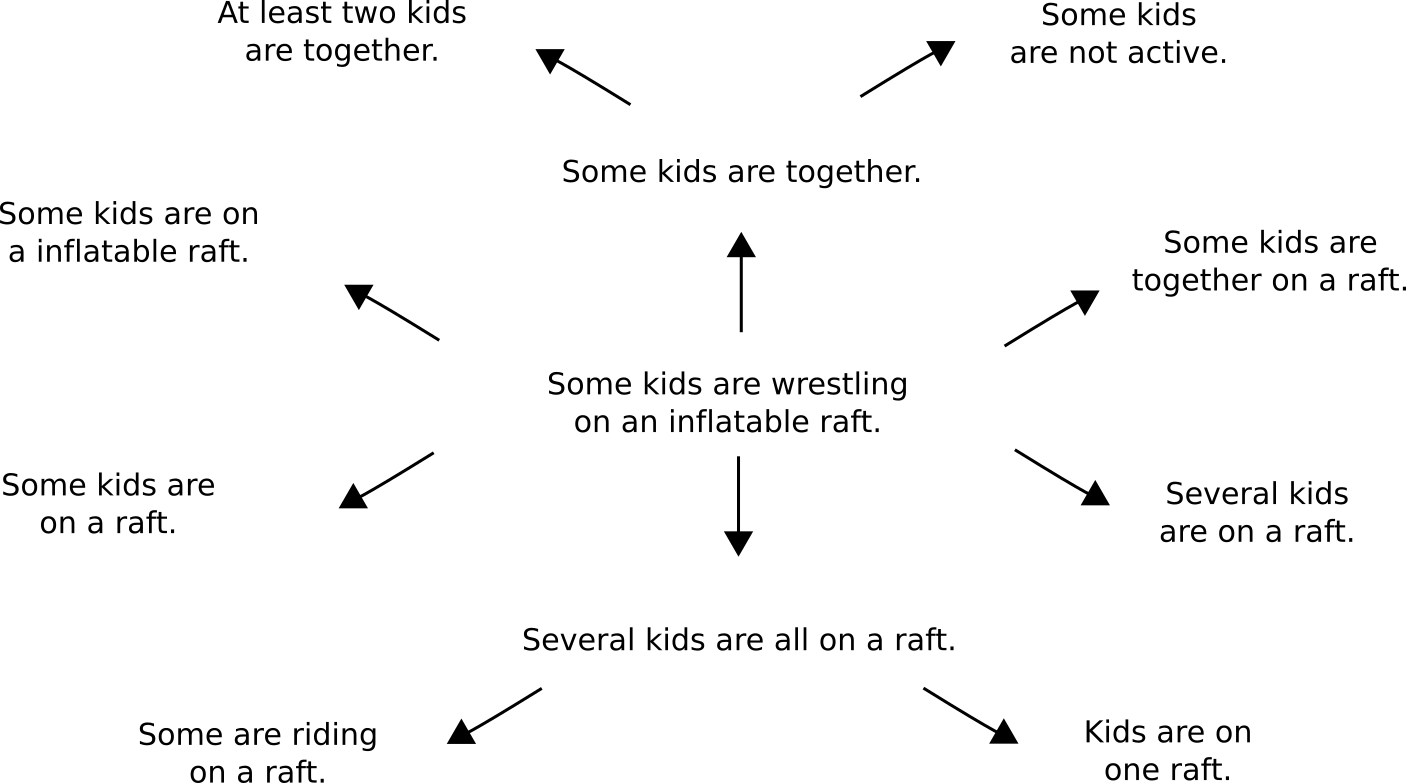
\includegraphics[width=5in]{figures/outward-inf-gen.png}
\end{center}
\caption{A model-generated inferential network around the sentence ``Some kids are wrestling on an inflatable raft.'' Each inferential transition is the result of generating a predicted entailment after encoding the sentence at the beginning of each arrow. The entire network is generated starting with only the initial sentence at the center of the diagram, which is drawn from the SNLI test set. Different decoding trees are used to generate the different entailments from the initial sentence.} 
\label{inf-gen}
\end{figure*}

Two general points can be made here. First, iterative applications of the model can be used to either generate sentences that are (a) increasingly specific, or (b) increasingly general \citep{Kolesnyk:2016}. If a predicted entailment is longer than the input sentence, then it tends to describe a more specific situation. For instance, the sentence ``A bird is in a pond'' can be used to generate the sentence ``A little bird is outside in a small pond'' by using a decoding tree with nodes for two additional adjectives and an additional adverb. If a predicted entailment is shorter than an input sentence, then it tends to describe a more general situation. For instance, the sentence ``A little bird is outside in a small pond'' can be used to generate the sentence ``A bird is outside'' by using a simple decoding tree with four nodes. 

Second, these capacities for specification and generalization suggest that the inferential transitions codified by the model can be either inductive or deductive in nature. For example, the inference from ``A bird is in a pond'' to ``A little bird is outside in a small pond'' is not strictly truth-preserving and therefore inductive. The inference from ``A little bird is outside in a small pond'' to ``A bird is outside'', on the other hand, \textit{is} strictly truth-preserving and therefore deductive. Interestingly, none of these inferences are formal in the sense that they are licensed strictly by the structure of the input sentence. Rather, they are examples of what Sellars (\citeyear{Sellars:1954}) and Brandom (\citeyear{Brandom:1994}) refer to as \textit{material} inferences, or inferences that are licensed solely by a linguistic expression's meaning. 

\begin{figure*}[t]
\begin{center}
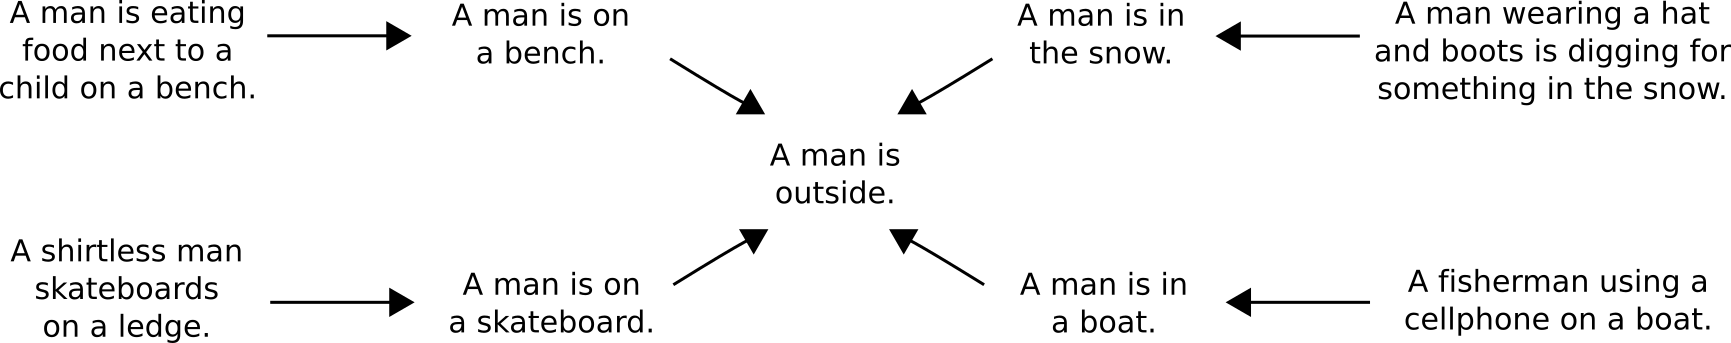
\includegraphics[width=6in]{figures/chain.png}
\end{center}
\caption{A model-generated inferential network around the sentence ``A man is outside''. Each inferential transition is the result of generating a predicted entailment after encoding the sentence at the beginning of each arrow. The entire network is generated starting with only the four outermost sentences, which are drawn from the SNLI test set.} 
\label{chain}
\end{figure*}

The most important lesson to draw from this examination of iterative prediction is that it illustrates how the model assigns an inferential role to every possible expression that can be formed from the words in its vocabulary. To explain, the model maps each input sentence onto a set of predictions concerning its inferential consequences. The model can then be used to map each sentence in this set to produce further predictions \textit{ad infinitum}. As such, it is possible to use the model to build networks of the sort shown in Figures \ref{inf-gen} and \ref{chain} for all possible input sentences. These networks, in turn, are explicit representations of the inferential roles the model assigns to particular sentences. Overall, since the model does not change as it is used to create these networks, it is fair to say that it defines an inferential role semantics for the entirety of the language that can be formed from the model's vocabulary. 

Of course, nothing guarantees that this semantics is appropriate for \textit{all} of the sentences in the language under consideration. It would be rather miraculous if a simple model trained on one hundred thousand entailment pairs managed to \textit{always} generate correct inferential transitions in novel scenarios. There is nonetheless some degree of fit between the inferential roles defined by this model and the inferential roles that govern the use of ordinary language. The goal of model development, then, is to steadily improve this degree of fit. Two changes are likely necessary to yield any substantial improvements. First, a much larger amount of training data must be made available to the model. The example inferential transitions in SNLI are somewhat idiosyncratic, and it is accordingly desirable to introduce training data that is reflective of the full range of inferential transitions that a competent language user would be inclined to make. Second, a more complex model architecture may be needed to take advantage of this additional training data. Neural networks are prone to ``catastrophic forgetting'' wherein the learning associated with newer training examples simply overwrites the learning associated with older ones. It is therefore possible that the specific model used in this experiment would not scale effectively with larger amounts of training data. Regardless, examining the use of different model architectures and larger amounts of training data is a task left for future research.

\subsection{Substitution Analysis}

Proponents of inferential role semantics typically characterize the meanings of individual words in terms of their effects on the inferential roles of the sentences in which they occur \citep{Brandom:1994,Brandom:2000,Block:1986}. The ``indirect'' inferential role associated with a particular word is then analyzed by swapping it into and out of a variety of different sentences to observe the resulting changes to the kinds of inferences that are licensed by these sentences \citep{Brandom:1994}. Interestingly, the model introduced here can be used to perform this kind of analysis in a quantitative manner. If individual words in the model's input sentence are replaced, it becomes possible to identify the impact these words have on the inferential transitions that the model predicts. In Table \ref{tab:sub}, for instance, the replacement of a subject noun or a main verb in an input sentence can be seen to have significant effects on the kinds of entailments that are generated by the model. 

\begin{table}[!t]
\begin{center} 

\caption{Substitution Analysis for ``A boy in a beige shirt is sleeping in a car''} 

\label{tab:sub}
\vskip 0.06in
\setlength{\tabcolsep}{12pt}
\begin{tabular}{ll} 
\hline

\multicolumn{1}{c}{\rule{0pt}{3ex} INPUT SENTENCE} & 
\multicolumn{1}{c}{GENERATED ENTAILMENT} \\

\hline
% \setlength{\tabcolsep}{1pt}
\rule{0pt}{3ex}A boy in a beige shirt is sleeping in a car. & A boy is sleeping in his car. \\
A girl in a beige shirt is sleeping in a car. & A girl is sleeping in her car. \\
A man in a beige shirt is sleeping in a car. & A man is sleeping in his car. \\
A woman in a beige shirt is sleeping in a car. & A woman is sleeping in her car. \\
A man in a beige shirt is driving in a car. & A man is driving a car. \\
A person in a beige shirt is selling a car. & A person is selling a car. \\
\hline
\end{tabular}
\end{center} 
\end{table}

There are two ways to think about the significance of this substitutional manipulation of the model's behavior. On the one hand, substitution can be used to assess how well the model is able to ``interpolate'' between the example inferential transitions it was trained on. To explain, any two sentences in the training data can be treated as substitutional variants of one another, provided that enough substitutions are made.\footnote{I include insertions and deletions, which can be thought of as substitutions involving the empty string.} For example, the sentence ``The dog chased after the cat'' is a substitutional variant of ``The woman drove the car'' -- ``dog'' is swapped for ``woman'', ``chased'' is swapped for ``drove'', ``after'' is swapped for the empty string, and ``cat'' is swapped for ``car''. If both of these sentences are part of inferential transitions found in the training data, then it is possible to evaluate how the model generalizes beyond these transitions by testing it on inputs that are the substitutional intermediaries of the original sentences. On the other hand, substitutions can also be used to identify specific inferential patterns that are associated with particular expression types (e.g., pronouns, quantifiers, etc.). Such patterns constitute what Brandom (\citeyear{Brandom:1994}) refers to as a subsentential expression's ``indirectly inferential role'' (p. 449). 

A main benefit of identifying indirect inferential roles is that many of the phenomena that semanticists have traditionally analyzed in truth-conditional terms can be re-analyzed in inferential terms. For example, one can test whether the model generates appropriate entailments for input sentences involving standard quantifiers like ``some'' and ``every.'' Similarly, one can test whether the model generates appropriate entailments for input sentences that exhibit anaphoric relations involving pronouns that vary with respect to gender and plurality (e.g., ``he'' vs. ``she'' vs. ``they'', etc.). Further tests involving expressions that vary with respect to numerals (e.g., one, two, many, etc.) are also possible. It is not reasonable to expect the model to pass all of these tests, since there are relatively few examples of inferential transitions in SNLI that are directly driven by quantification, anaphora, or numerosity. Nonetheless, the model exhibits some promising behavior with respect to these expression types.

In the case of quantifiers, the model is able to infer that ``some'' and ``many'' require nouns within their scope to take the plural form in an entailed sentence, as shown in Table \ref{tab:quantifiers}. The model is also able to infer that ``some'' entails ``at least one'', as shown in Figure \ref{inf-gen}. In the case of pronouns, the model is sensitive to cues that determine the gender of a pronoun in relation to its anaphoric antecedent. For example, the model correctly infers that girls and women should be referred to with female pronouns, while boys and men should be referred to with male pronouns, as shown in Table \ref{tab:sub}. In the case of numerals, the model exhibits an ability to infer appropriate quantities from simple groupings and conjunctions. For instance, the model generates a sentence containing the phrase ``Two kids...'' from a sentence containing the phrase ``A boy and a girl...'' in Table \ref{tab:quantifiers}. Finally, the model appears to have difficulty with negations. In Table \ref{tab:quantifiers}, for example, the model incorrectly infers ``A boy is not indoors'' from ``A boy in a red shirt is waiting in a store.'' While these results are rather limited, it is worth emphasizing again that the model was not designed or trained to account for phenomena involving quantifiers, pronouns, and numerals specifically. So the fact that the model's predictions are appropriately sensitive to these expressions in some cases suggests that it provides a solid foundation for developing more sophisticated analyses of specific linguistic constructions. 

\begin{table}[!t]
\begin{center} 
\caption{Substitution Analysis with Quantifiers, Numerals, and Negations} 
\label{tab:quantifiers} 
\vskip 0.06in

\setlength{\tabcolsep}{13pt}
\begin{tabular}{ll} 
\hline

\multicolumn{1}{c}{\rule{0pt}{3ex} INPUT SENTENCE} & 
\multicolumn{1}{c}{GENERATED ENTAILMENT} \\

\hline
\rule{0pt}{3ex} Some men in red shirts are waiting in a store. & \quad The men are in a store. \\
Many women in red shirts are waiting in a store. & \quad The women are in a store. \\
A boy and a girl are waiting in a store. & \quad Two kids are indoors. \\
A boy and a girl are waiting in a playground. & \quad Two kids are outside. \\
A boy in a red shirt is sleeping in a car. & \quad A boy is not outside. \\
A boy in a red shirt is waiting in a store. & \quad A boy is not indoors. \\
\hline
\end{tabular}

\end{center} 
\end{table}

Overall, the extent to which this sort of substitutional analysis can be used to define the meanings of individual words is an open question. Words are typically only used in the context of sentences, and sentences, I have argued, have meanings insofar as they license certain inferences. It is accordingly plausible that words have meanings insofar as they help determine which inferences are licensed by the sentences they occur in. Strictly speaking, I endorse this line of reasoning, but it can be misleading if one only considers inferences that relate linguistic expressions to one another, to the exclusion of inferences that relate linguistic expressions to non-linguistic perceptions and actions. In the case of a word like ``crayon'', for instance, it would be inadequate to postulate a meaning that merely codifies inferential relations amongst crayon-related sentences while saying nothing about how people identify and use crayons. A more detailed discussion of this topic is provided in Chapter 6, but for now, suffice it to say that purely linguistic inferential roles of the sort formalized in this chapter are at the very least a necessary component of an expression's meaning.

\subsection{Conditioned Entailments}

Up to this point, the association of particular inferential roles with particular sentences has not lead to any concrete explanations of facts concerning the \textit{use} of these sentences. To build towards such explanations, I briefly examine various methods for conditioning the model's predictions on additional inputs. The idea is to selectively navigate the inferential role associated with a particular sentence so as to provide appropriate answers to specific questions about the sentence. To illustrate with a hypothetical example, consider the sentence that was used to motivate the predictive adequacy criterion in Chapter 1: ``The boy waited for the pitch and then hit the ball over the fence.'' Providing an answer to a question such as ``Where did the ball go?'' or ``What did the boy likely use to hit the ball?'' involves drawing one inference amongst the many that are licensed by the original sentence. More generally, every answer to a question about this particular sentence is simply a different sentence specified by its inferential role.

\begin{table}[!t]
\begin{center} 
\caption{Prompts with ``A shirtless man sleeps in his blue boat out on the open waters''} 
\vskip 0.15in
\label{prompt} 

\setlength{\tabcolsep}{25pt}
\begin{tabular}{ll} 

% \multicolumn{2}{c}{SENTENCE: \quad A shirtless man sleeps in his blue boat out on the open waters.} \\
\hline

\rule{0pt}{3ex} PROMPT & \qquad \qquad \quad GENERATED ENTAILMENT \\

\hline
% \setlength{\tabcolsep}{1pt}
\rule{0pt}{3ex}\quad Water & \qquad \qquad A shirtless man is in the blue water.\\
\quad Blue & \qquad \qquad A blue man is in the blue boat. \\
\quad Fishing & \qquad \qquad A shirtless man fishing in the blue water. \\
\quad Sleep & \qquad \qquad A shirtless man sleeps in the blue water. \\
\quad Boat & \qquad \qquad A shirtless boat boat in the blue boat. \\
\hline
\end{tabular}
\end{center} 
\end{table}

There are two reasons why question answering is worth exploring in detail. First, the matter of whether a model can adequately perform simple forms of question answering is highly relevant to determining whether or not it can be appropriately described using the vocabulary of intentional systems theory. Put simply, a system that \textit{understands} a particular linguistic expression will undoubtedly be able to answer certain questions about it. Given that I argued in Chapter 1 that the expectations set out by inferential roles are what make intentional interpretation possible,\footnote{The idea, recall, is that intentional state attributions only license certain behavioral predictions because the sentences invoked by these attributions have particular inferential roles.} it is important to verify that my model can be subjected to such interpretation. Second, an examination of question answering allows for a clear connection to be drawn between the inferential roles assigned to particular expressions and the \textit{use} of those expressions. For example, the assignment of an inferential role to a sentence suffices to explain, amongst other things, how it gets used in simple question-and-answer dialogues.

As an initial test of the model's ability to generate conditioned entailments, I supplement its input with simple prompts consisting of single words. The resulting change to the encoding procedure is quite minimal. First, an input sentence is converted into an embedding using the usual tree-structured encoder. Second, a word embedding corresponding to a prompt is added to this embedding. The resulting sum is then passed through the decoder to produce a predicted entailment. The effect of this process is to subtly shift the input sentence embedding towards the prompt embedding in the hope that this shift will be reflected in the prediction of an entailment that is appropriate to the prompt. Table \ref{prompt} illustrates some examples of the kinds of the entailments that the model predicts under these conditions.  

The natural next step is to use complete questions instead of single word prompts to condition the model's predictions. To take this next step, I simply modify the encoding procedure to produce \textit{two} sentence embeddings using two separate encoding trees. The first embedding corresponds to an input sentence, while second embedding corresponds to a question. These embeddings are then simply added together before being passed to the decoder network. The hope, again, is that shifting the input embedding towards the question embedding will force the decoder to predict and entailment that is an answer to the question. An important caveat is that the model was not trained to perform this task, so there is little reason to suppose that it will produce appropriate answers. As Table \ref{query} indicates, the answers the model provides in response to questions are often not particularly illuminating or coherent. Nonetheless, these answers are occasionally on the right track, as in the case of the first example in the table.

\begin{table}[!t]
\begin{center} 
\caption{Queries with ``A mother and daughter walk along the side of a bridge''} 
\label{query} 

\vskip 0.07in
\setlength{\tabcolsep}{8pt}
\begin{tabular}{ll} 

% \multicolumn{2}{l}{SENTENCE: \qquad \quad A mother and daughter walk along the side of a bridge.} \\
\hline

\rule{0pt}{3ex} QUERY &  GENERATED ENTAILMENT \\

\hline
% \setlength{\tabcolsep}{1pt}
\rule{0pt}{3ex}How many people are walking? & Two people are walking.\\
 Are the mother and daughter walking? & The mother and daughter walking outdoors.  \\
 What is the bridge over? & A people are on the bridge. \\

\hline
\end{tabular}
\end{center} 
\end{table}

Overall, these tests are merely suggestive, but they point towards the development of more sophisticated models for which performance on conditional inference tasks is incorporated directly into the training objective. Developing such models will undoubtedly require training data comprised of numerous example question-answer pairs for each input sentence of interest. There are currently a number of engineering-driven efforts to build systems that learn to answer questions about short collections of text \citep[e.g.,][]{Weston:2015,Weston:2016,Sukhbataar:2015}, but these efforts have not lead to the creation of publicly available datasets of the required sort.

\section{Consequences for Semantic Theory}\label{sec:consequences}

Collectively, the experiments just described paint a somewhat mixed picture of the model's performance. On the one hand, the model is able to predict appropriate entailments for a wide range of novel sentences. There is accordingly a clear sense in which the model satisfies the goal of ``making explicit'' the inferential roles of these sentences. On the other hand, the model struggles to generate entailments that are appropriately sensitive to the presence or absence of certain subsentential expressions. The model also struggles to selectively generate entailments in response to specific prompts and questions. These shortcomings are important because they demarcate the limits within which the intentional stance is predictive of the model's behavior. To explain, the model can be attributed a very rudimentary understanding of certain linguistic expressions, but it clearly cannot be attributed the full-fledged understanding possessed by a competent language user. It is a system that, in Dennett's terms, only ``sort of'' understands the sentences it is presented with \citep[qtd. in][]{Rothman:2017}.

``Sort of'' understanding a sentence is not nothing, but neither is it everything. So it is worth considering what further characteristics the model would need to possess in order to count as a full-fledged comprehender, or an intentional system comparable in nature to a linguistically competent human being. Arguably, these further characteristics fall into three general categories. First, true comprehenders are able to draw appropriate inferences on the basis of multiple pieces of information. If, for example, a person is told a simple story, they will be able to draw inferences about this story as a whole. So a model that understands language would similarly need to be able to draw ``multi-premise'' inferences involving simple narratives. Second, true comprehenders are able to draw inferences that involve non-linguistic perceptions and actions. If, for example, a person is told that a wet dog is in the house, they will expect to see drops of water on the floor. So a model that understands the sentence ``A wet dog is in the house'' would similarly need to be able to relate this sentence to certain non-linguistic observations. Finally, true comprehenders are able to effectively deploy language in a wide variety of conversational scenarios. They can ask and answer questions, respond to directions, and provide instructions, along with many other things. So a model that understands language would similarly need to be able \textit{use} language effectively in all such contexts.

It is useful to briefly speculate on some strategies for introducing these characteristics into a model. In the case of multipremise inferences, one option is to provide the model with a memory to store information about multiple sentences. The generation of an entailment could then be conditioned on \textit{all} of the sentences stored in the memory, rather than just a single sentence. A variant of this basic strategy has been developed in the recent machine learning literature on question answering systems, wherein ``memory networks'' are used to store information about simple stories and then answer certain questions amount them \citep{Weston:2016,Weston:2015,Sukhbataar:2015}. One drawback of this research is that it is not motivated by theoretical concerns about semantics. Rather, it is driven primarily by engineering considerations.

In the case of inferences that involve non-linguistic perceptions and actions, one option is to provide the model with a visual system that converts images into embeddings that can then be passed through the decoder to generate a predicted entailment. Likewise, one could provide the model with a motor system that uses sentence embeddings to generate specific actions. The idea in both cases is to extend the model to perform what Sellars (\citeyear{Sellars:1954}) refers to as ``language-entry'' and ``language-exit'' transitions, which are distinct from the ``language-language'' transitions formalized here. Interestingly, there are a number of available templates for building models that account for these further transitions. Socher et al. (\citeyear{Socher:2014}), for instance, describe a model that uses a tree-structured neural network in tandem with a convolutional neural network to match images to linguistic descriptions of their contents. On more a cognitive level, Eliasmith et al. (\citeyear{Eliasmith:2012}) describe a neurocomputational model that performs a variety of tasks that involve responding to visual images with specific motor behaviors. There are accordingly a number of tools available for building models that codify complex inferential roles spanning the domains of language, perception, and action. 

Finally, in the case of inferences that guide conversational activity, the obvious strategy is to first provide the model with the ability to perform a range of actions and then develop a training paradigm in which the model learns to perform specific actions in specific situations. For instance, the model could learn an action policy for which questions are responded to with answers, while commands are responded to with actions that fulfill them. The idea, in short, would be to construct a model that learns to make the moves involved in a variety of different ``linguistic dances.'' There are some basic templates for this sort of research. For example, reinforcement learning techniques have recently been used to build models that learn highly complicated action policies for accomplishing certain goals \citep{Mnih:2015}. It is conceivable that analogous policies could be learned for carrying out the kinds of cooperative joint actions that are fundamental to language use.

Overall, there is no easy way to build a model of the sort I am envisioning, yet it is instructive to imagine it. By hypothesis, the model would be a genuine intentional system, capable of understanding language at a human-like level, and of playing the ``game of giving and asking for reasons'' \citep{Brandom:1994}. Now consider a question: if this model provides a complete formal specification of the role that a given linguistic expression plays in regulating its behavior, would there be any facts about the \textit{meaning} of this expression that the specification leaves out? On the assumption that the model's behavior is that of a competent language user, it is plausible that there are no such facts. Put simply, if one has an explicit definition of the role that a particular linguistic expression plays in determining the behavior of intentional systems that use it, then one has an explanation on hand of all relevant facts concerning the expression's use. The definition would thereby satisfy the explanatory goals of semantic theory outlined in Chapter 1. 

\section{Conclusion}

In summary, the point of this work is to motivate an approach to semantics based on inferential relationships \citep{Brandom:1994}. The use of the encoder-decoder model is designed to illustrate how generalized inferential roles can be learned for arbitrary linguistic expressions from examples of how sentences are distributed as tacit ``premises'' and ``conclusions'' in a space of inferences. It is accordingly possible to characterize this work as an extension to the well-known distributional approach to semantics \citep{TurneyPantel:2010}, wherein the generic notion of a linguistic context is replaced with the more fine-grained notion of an inferential context. 

As with most natural language generation systems, many of the sentences produced by the model are defective in some way. As can be seen in the examples in Tables \ref{prompt} and \ref{query}, model-generated entailments are almost always thematically appropriate, but sometimes contain agreement errors or misplaced words that render the entailment as a whole ill-formed. And, not infrequently, the model produces entailments that are more or less incomprehensible. There are two ways to address these problems. The first involves the use of increased amounts of training data to provide the model with a more points in the ``space of inferences'' to interpolate between. The second involves the use of more sophisticated network architectures that help the model to learn to more selectively make use of only the input information that is most relevant to generating a good entailment. LSTM network architectures, such as the Tree LSTM \citep{Tai:2015}, are likely to provide improvements on this second front. 

Finally, an important limitation of this work is that it does not directly consider the relationship between linguistic expressions and the non-linguistic world. A natural way to account for this relationship is to suppose that a sentence's occurrence in the linguistic environment licenses certain expectations about what can be seen, heard, or otherwise perceived. To return to my initial example, if one understands the statement ``The dancers parade down the street'', one will expect to see and hear dancers upon going to the relevant street. I accordingly suggest that if an individual can adequately infer all that follows from a given linguistic expression, both linguistically and non-linguistically, then there is nothing further they need to be able to do to count as \textit{understanding} what the expression means.

